\documentclass[11pt, letterpaper]{article}
\usepackage[letterpaper, margin=1in]{geometry}

\usepackage[hidelinks]{hyperref}
\usepackage{graphicx}
\usepackage{enumitem}

\begin{document}

\begin{titlepage}
  \begin{center}
      \vspace*{1cm}
      
      \fontsize{18}{18}\textbf{Modern Single Object Tracking Methods:} \\
      \fontsize{18}{18}\textbf{A Comprehensive Literature Review}
      
      \vspace{0.5cm}
      Presented by \\
      Santam Bhattacharya, Riley Eaton, Dichen Feng, Wanju Luo, Henry Pa
      
      \vfill
          
      COSC 444/544: Computer Vision \\
      University of British Columbia \\
      Kelowna, BC \\
      \today
          
  \end{center}
\end{titlepage}

% -------------------------- ABSTRACT --------------------------
\clearpage
\section{Abstract}

Computer vision enables machines to interpret visual data, with single object tracking (SOT) being a key challenge for applications like robotics and autonomous vehicles. SOT involves tracking a specific target across video frames but is complicated by issues such as occlusion and fast motion. While traditional methods like correlation filters and modern deep learning approaches have advanced tracking, they still face limitations. This literature review examines these methods and their shortcomings. Our proposed approach combines multiple tracking models—MOSSE, CCOT, SRDCF, and KCF—into an ensemble, allowing each model to contribute to improved tracking performance. We anticipate this method will offer a more robust and adaptable solution to SOT challenges.


% -------------------------- INTRODUCTION --------------------------

\section{Introduction}

Computer vision is a rapidly advancing area of artificial intelligence that enables machines to interpret and understand visual data, much like human vision. It encompasses a wide range of tasks, including object recognition, image segmentation, scene reconstruction, and motion tracking. Among these tasks, single object tracking (SOT) presents a fundamental challenge. In SOT, the goal is to track a specific target across a sequence of video frames, which is essential for applications such as autonomous vehicles, robotics, surveillance, and traffic monitoring. The ability to accurately track a target in real time is critical for the functionality of these systems in dynamic environments.

SOT is particularly relevant in detection-free tracking, where the target object's initial position is manually set in the first frame, and the tracker continues to follow it in subsequent frames without the need for re-detection. While this approach offers flexibility, it is not without its challenges. Real-world scenarios often present difficulties such as occlusion, changes in lighting, fast motion, and target deformation. These factors make SOT a complex and ongoing research problem, with significant implications for practical systems that require reliable and robust tracking.
To tackle these challenges, a thorough review of existing methods is essential to understand the strengths and weaknesses of current SOT approaches. Traditional methods, such as correlation filters, have been significantly improved through the integration of deep learning techniques. These advancements have led to notable gains in tracking performance, yet issues like handling occlusions and fast motion remain areas of active research.

This literature review will focus on the evolution of SOT techniques. It will cover the main steps in SOT—feature extraction, candidate generation, model building, and updating—highlighting advancements in correlation filters and deep learning-based methods. Current research focuses on improving feature extraction, model compression, and unsupervised tracking. Challenges such as occlusion, deformation, scale transformation, and fast motion continue to drive ongoing SOT research.
Our proposed approach aims to build on these existing methods by combining multiple tracking models—MOSSE (Minimum Output Sum of Squared Errors), CCOT (Continuous Convolution Operators for Tracking), SRDCF (Spatially Regularized Discriminative Correlation Filter), and KCF (Kernelized Correlation Filter)—into a single ensemble model. By leveraging the strengths of each model, we aim to create a more robust and adaptable solution that can improve tracking accuracy, particularly in scenarios involving occlusion and fast motion. This ensemble approach holds the potential to offer a more generalizable and reliable solution for real-world tracking challenges.

% -------------------------- RELATED WORKS --------------------------
\section{Related Works}
\subsection{Template Matching}

Template matching uses the initial image patch of the target object as a template and searches for the best match of this template in subsequent video frames. Two common similarity measures used in template matching are Normalized Cross-Correlation (NCC) and Sum of Squared Differences (SSD). NCC is more robust against illumination changes but computationally expensive, while SSD offers lower computational cost but is less resilient to lighting variations. The process typically slides the template over the search area pixel by pixel, computing a similarity metric at each position. The location with the highest similarity score is considered the new position of the target. While the method being computationally efficient and easy to implement, the method works best for targets with consistent appearance and is less robust to significant changes in scale, rotation, or partial occlusions. 

\subsection{Feature-Based Tracking}

These foundational methods for object tracking focus on distinct target features, as opposed to entire regions such as in template matching. This allows for more robust tracking when dealing with slight changes in pose, lighting, and partial occlusion of targets.

\subsubsection{Histogram of Oriented Gradients}

One notable example of this technique is the Histogram of Oriented Gradients (HOG), which aims to capture the shape and appearance of an target using edge directions. For each image, the gradient magnitude and orientation at each pixel are calculated. These represent the direction and strength of intensity changes, which correspond to the edges in the image. Then, the image must be split up into small cells, where each cell stores the number of gradient orientations within it, in a histogram. These histograms can then be linked together to form a feature descriptor, capturing the shape and texture of the target. This deeper understanding of the target's shape allows it to better deal with lighting changes, but makes it ineffective for targets that experience pose variations.


\subsubsection{Scale-Invariant Feature Transform}

The Scale-Invariant Feature Transform (SIFT) is another feature-based method that was introduced to better detect objects with variations in lighting, viewpoint, and all forms of translation \cite{lowe_object_1999}. It relies on keypoint detection, which are points in an image across different scales, and selected by searching for local extrema in the Difference-of-Gaussians (DoG) scale space. This allows SIFT to be very effective at detecting a target that experience scale changes. The filtered keypoints are then grouped into neighbourhoods, and assigned an orientation based on the local gradients within. This is done to create an accurate descriptor for robust object detection when rotation occurs. One disadvantage to this approach is evident when targets experience non-rigid deformations, as they cause distortions in the fixed-size keypoint neighbourhoods. Additionally, and similarly to HOG, SIFT relies on gradients, which means that it will be less effective in regions with little texture. Overall SIFT is an excellent method for object detection, however due to its lack of design for tracking it is very computationally expensive for single object tracking (SOT), and therefore has many better alternatives as will be discussed. 

\subsection{Correlation Filters}

As we move into more contemporary approaches to SOT, we begin to approach the state-of-the-art (SOTA). These methods build upon previously established computer vision techniques to advance tracking through improvements in performance and efficiency, when compared to traditional methods. There are hundreds of SOTA methods in the domain of SOT, many of which are evolving by the day. Because of this, we will be focusing on a few specific methods that make use of powerful, modern approaches to SOT.
The first modern methods we will discuss are bared on correlation filter (CF) tracking. This is a technique used for tracking whereby the process of learning the target's appearance is framed as a convolution problem in the frequency domain. This involves convolving the filter and the image, similar to the similarity measure in template matching. Frequency domain computations are used to increase the computational efficiency of the correlation (similarity measure) between the filter and the image. Typically, a Fast Fourier Transform (FFT) is used to convert the image and filter into the frequency domain. Once the necessary computations have been performed, the inverse FFT (iFFT) is used to return the results in the original, spatial domain. This efficiency boost is best realized in high frame rate applications, as seen in most real-time environments \cite{noauthor_visual_2010}.

\subsubsection{Discriminative Correlation Filters and Spatial Regularization}

Discriminative correlation filter (DCF) tracking builds upon previous CF trackers, with the key distinction of treating correlation filtering as a supervised learning problem. This is done by training on both positive and negative samples, where negative samples represent anything except the target to be tracked. This approach maintains high precision in challenging environments, such as occlusions, distractors, and variations in appearance. Although DCFs have proven useful in these scenarios, they have traditionally suffered when boundary effects are present \cite{zhu_efficient_2021}. These effects can occur when broken or noisy edges are present, and when dealing with complex or changing boundary shapes and textures. This is due to various inherent compromises of DCFs, such as the confined search region, and the potential for overfitting due to the lack of diversity in negative (background) training samples. To address these issues, Spatially Regularized Discriminative Correlation Filters (SRDCF) were proposed for SOT \cite{danelljan_learning_2015}. As the name indicates, this approach introduces spatial regularization, which spatially penalizes the CF weights. Due to the spatial nature of these new weights, they are easily understood when visualized. An excellent example of this is provided in the original work, as seen in Figure \ref{fig:spatial_weights}.

This applied regularization results in filter values with less spurious noise in background regions, and is visualized in Figure \ref{fig:spatial_weights_compared}, taken from the original work. As can be seen, the resulting regularized weights place more emphasis on the positive region of the image (to be detected), which leads to an improvement in the model's ability to discriminate between positive and negative samples. This is especially true where the spatial window is small, which can occur with boundary effects. Overall, the improved discriminative ability of a model is directly linked to its detection performance, therefore model accuracy increases when using SRDCF over DCF. 

One notable drawback of SRDCF is its use of a fixed spatial regularization window for tracking. This puts SRDCF at a disadvantage in situations where the scale of a target changes. If a target becomes too small in comparison to the pre-determined window, then the regularization will give more weight to some irrelevant features within the window. On the other hand, if a target expands too much, then the useful target features that fall outside the window will be suppressed. Either of these situations will lead to a decrease in the model's performance.

\begin{figure}
  \centering
  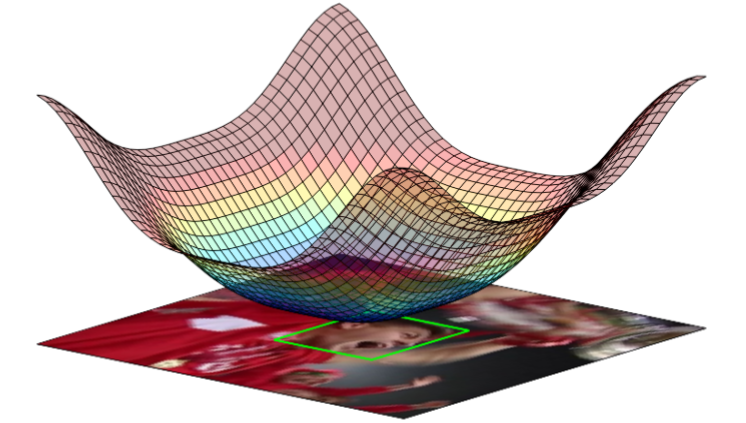
\includegraphics[width=0.6\linewidth]{img/spatial-weights.png}
  \caption{\label{fig:spatial_weights}\textit{Visualization of the spatial weights used by SRDCF (during learning), shown above the image used for training, where the green highlighted region represents the positive (correct) detection \cite{danelljan_learning_2015}.}}
\end{figure}

\begin{figure}
  \centering
  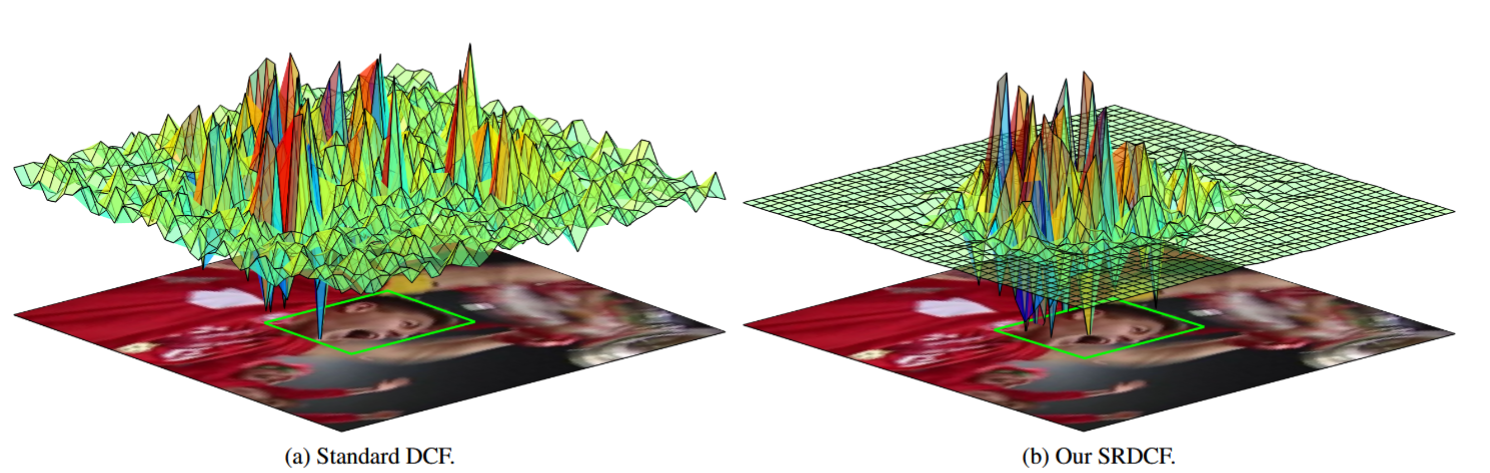
\includegraphics[width=1\linewidth]{img/spatial-weights-compared.png}
  \caption{\label{fig:spatial_weights_compared}\textit{Comparison of filter weights between standard DCF and SRDCF, shown above the image used for training, where the green highlighted region represents the positive (correct) detection \cite{danelljan_learning_2015}.}}
\end{figure}

\subsubsection{Kernelized Correlation Filters}

Kernelized Correlation Filters (KCF) is a nonlinear method which combines correlation filters with kernel methods. There the solution is obtained in a nonlinear feature space exploiting the kernel trick. KCF operates in the frequency domain to significantly improve the processing speed. It also includes different types of features (e.g., HOG, colour channels), which are fused in the Fourier domain using DFT-based computation. Benefits associated with more complex feature representations include more robustness to changes in illumination, occlusions, and other deformations. On the other hand, naturally, using more complex feature representations results in additional computational overhead when online training is performed \cite{chumachenko_chapter_2022}. One key drawback that is seen in many CF trackers such as KCF is the use of a fixed template size, which leads to a lack of adaptability when the target changes size. However, as mentioned KCF excels in dealing with targets that experience illumination changes and occlusions.

\subsubsection{The Minimum Output Sum of Squared Errors}

The Minimum Output Sum of Squared Error (MOSSE) tracker is a landmark method in correlation filter-based tracking that offers high-speed performance and simplicity. It differs from traditional template matching by learning an adaptive filter in the frequency domain, which is updated online to accommodate changes in the target's appearance.

Instead of using a fixed template, MOSSE generates a Gaussian response for the selected target and creates multiple synthetic training samples by applying random warps. The filter is computed in the Fourier domain as:

\begin{equation}
  H = \frac{A_i}{B_i}
\end{equation}

Where $A_i$ and $B_i$ are accumulators obtained from the Fourier transforms of the warped samples and the Gaussian response.

The MOSSE tracker offers several advantages, including high-speed performance by leveraging the Fast Fourier Transform (FFT), simplicity with a straightforward implementation and low computational footprint, and adaptability through online updating to maintain tracking accuracy over time. However, it also has some limitations. The tracker operates at a fixed scale, making it less effective for targets with significant size variations. Its performance may decrease when the target is partially or heavily occluded, and the fixed update strategy may cause gradual tracking error accumulation under challenging conditions.

\subsubsection{Continuous Convolution Operators}

The Continuous Convolution Operators Tracker (C-COT) is a visual tracking framework that learns continuous convolution filters for both object tracking and feature point tracking. C-COT introduces a novel formulation for learning convolution operators in the continuous spatial domain, enabling the estimation of a target's trajectory in a video. C-COT can efficiently integrate multi-resolution deep feature maps, overcoming the single-resolution limitation of conventional Discriminative Correlation Filter (DCF) formulations. By labelling training samples with sub-pixel precise continuous confidence maps, C-COT enables accurate sub-pixel localization, which is crucial for accurate feature point tracking. C-COT is a discriminative learning-based approach that does not require explicit interpolation of the image to achieve sub-pixel accuracy. For training, C-COT uses the Conjugate Gradient method, which scales linearly with the number of feature channels, making it suitable for high-dimensional deep features \cite{danelljan_beyond_2016}.

\subsection{Scale Space Tracking}

Scale space tracking has become an essential technique in object tracking to account for changes in target size. As discussed, many early correlation filter-based trackers, such as MOSSE and KCF, rely on the assumption of a fixed target scale, which limits their performance in dynamic environments. The Discriminative Scale Space Tracker (DSST) addresses this limitation by introducing a dedicated scale filter alongside the traditional translation filter, enabling simultaneous tracking of both target position and size. By performing scale adaptation in a discriminative manner, DSST effectively handles challenges like target resizing and partial occlusions. This method has led to significant improvements in the accuracy and robustness of tracking algorithms, influencing the development of later trackers that integrate both scale and translation filtering for more reliable performance in real-world applications \cite{danelljan_discriminative_2017}.

\subsection{Ensemble Models for Visual Tracking}

There is limited research on ensemble models for object tracking tasks. One of the prominent studies, conducted by Du, Yunhao, et al. \cite{du_ensemblemot_2023}, proposed EnsembleMOT to merge multiple tracking results from various trackers using spatio-temporal constraints. Cobos, Hernandez, and Abad \cite{cobos_fast_2019} present a fast multi-object tracking system that utilizes an ensemble of object detectors, each running every fff frames, combined with a variation of the Soft-NMS algorithm to increase prediction performance while maintaining real-time capabilities.

% -------------------------- PROPOSED METHOD --------------------------
\section{Proposed Method}

\subsection{Problem Statement}

As highlighted in section 3, the key barriers to effective single object tracking (SOT) are when the target object experiences significant variations such as in scale, position, lighting, occlusions, pose, and other deformations. Many approaches have been proposed to increase model efficiency in each these scenarios, however with every area of improvement comes an area where efficiency is sacrificed.

\subsection{Core Ideas}

The proposed model will ensemble the MOSSE, C-COT, KCF, DSST and DCF. As has been explored, the various approaches in section 3 prove their effectiveness in a specific SOT scenario. Because of this, we propose a method to address the key barriers to effective SOT through the development of an ensemble model. Ensemble models have been proven to be effective in many areas of machine learning, where the resulting model is more accurate and robust than any one of its constituents, given the same task.

\subsection{Technical Details}

The proposed model will explore the two different ways—Stacking and Voting—to ensemble the MOSSE, C-COT, KCF, DSST and DCF.
For voting strategy, each independent model will get a representation by contributing its tracking results. Firstly, it runs each tracker on the input video to generate predictions, such as bounding boxes or keypoints, for each frame. Next, it aggregates the predictions by applying a voting mechanism where each tracker "votes" for the object's position in each frame, either through \emph{majority voting} or \emph{weighted averaging} based on tracker reliability. Finally, the model outputs the most common or consistent prediction as the final tracking result for each frame, ensuring that the ensemble method leverages the strengths of diverse trackers to improve robustness and accuracy in various tracking scenarios.

The stacking strategy will combine predictions from multiple SOT models to improve tracking performance. The process begins by training several base models mentioned above, each capable of tracking the object in a video using different methods. Each tracker produces a set of predictions (bounding boxes or keypoints) for the object's position in each frame.
Once the base models are trained, their outputs are used to form a meta-feature set. This set consists of the predictions (bounding boxes, confidence scores, velocities, etc.) from each base model, which are then combined into a feature vector for each frame. These feature vectors are used as input to a meta-model, such as logistic regression or support vector machine (SVM), which learns to combine the base model outputs into the best possible prediction of the object's position.

After training, the meta-model can make final predictions by using the stacked feature set from the base models on new data. The meta-model evaluates the combined predictions to produce a more accurate and robust result. Stacking helps to improve accuracy by leveraging the strengths of multiple trackers, making the ensemble more resilient to challenges that any single tracker might struggle with, such as occlusions, motion blur, or background clutter.

\subsection{Initial Experiments}

Thus far, we have replicated each individual model separately. OTB2015 and LaSOT are chosen as the benchmark for the research.

\subsubsection{Benchmark}

Our research uses OTB2015 and LaSOT for benchmark. OTB2015 is a standard dataset used for tracking testing, consisting of 100 fully annotated sequences divided into 11 attributes based on content. Common evaluation metrics for this benchmark are success plots and precision plots, with AUC and precision score at a threshold of 20 pixels being key indicators \cite{otb_2015_papers_nodate}. Top performing models for visual object tracking using this dataset can be seen in Figure \ref{fig:otb2015}. Meanwhile, LaSOT is a large-scale, high-quality SOT dataset containing 70 categories, each with 20 sequences averaging 2,512 frames, resulting in approximately 3.52 million high-quality bounding box annotations. Evaluation metrics include precision, normalized precision ($Pnorm$), and success (AUC), with $Pnorm$ accounting for the impact of object scale and image resolution \cite{lasot_papers_nodate}.

\begin{figure}
  \centering
  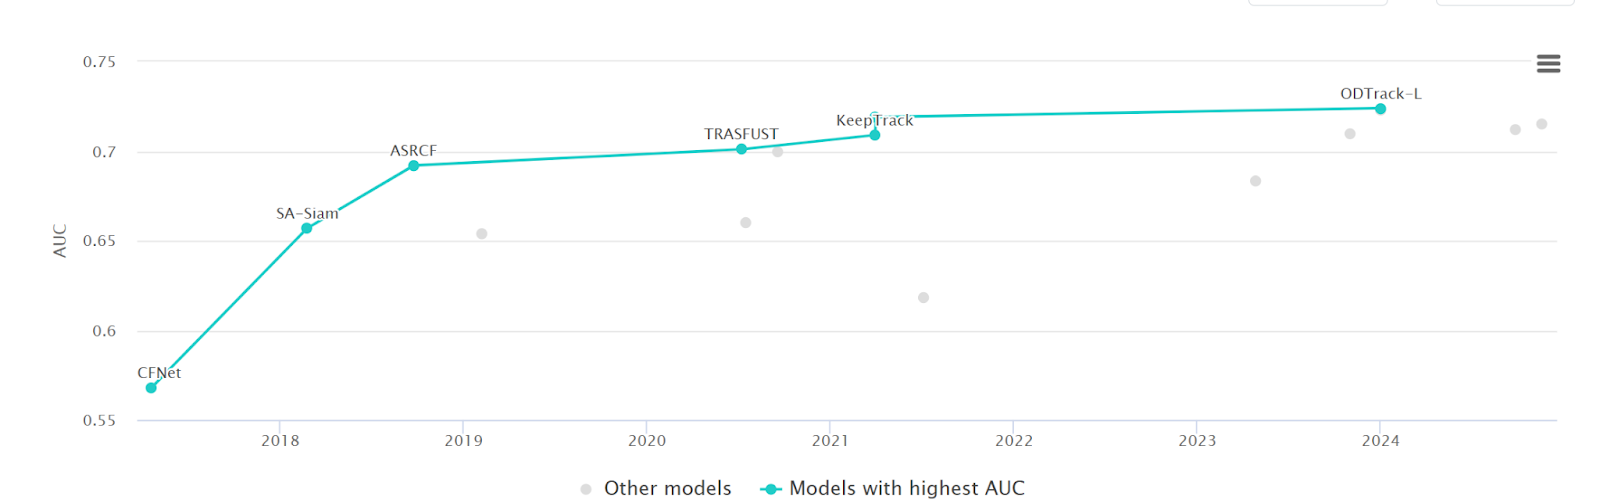
\includegraphics[width=1\linewidth]{img/otb2015.png}
  \caption{\label{fig:otb2015}\textit{Visual Object Tracking on OTB-2015 \cite{otb_2015_papers_nodate}.}}
\end{figure}

\subsubsection{KCF Replication}

In our current work, we aim to replicate each of the constituent models in the ensemble, thus far we have replicated KCF, and MOSSE. The open-source implementations of SRDCF are sparse, so we are attempting to replicate a newer variant, the STRCF \cite{li_learning_2018} with source code available at \underline{\href{https://github.com/lifeng9472/STRCF}{https://github.com/lifeng9472/STRCF}}. The MOSSE tracker was replicated through a MATLAB implementation. The code reads a sequence of image files (each representing a frame), allows the user to select the target in the first frame, generates a Gaussian template, creates synthetic training samples via random warping, and computes the adaptive filter in the frequency domain. The tracker then applies this filter frame by frame, updating it online to maintain robust tracking. For KCF replication, the target is selected using a manual bounding box (Figure \ref{fig:kcf_select}) and then tracks the target's position as it updates (Figure \ref{fig:kcf_updates}) with the following configuration:

\begin{enumerate}
  \item \textbf{Input:} Video frames.
  \item \textbf{Feature Extraction:} HOG and grayscale features.
  \item \textbf{Filtering Computation:} Kernelized Correlation Filtering.
  \item \textbf{Target Position Update:} Adjust the model with confidence evaluation.
  \item \textbf{Output:} Updated target position.
\end{enumerate}

\begin{figure}
  \centering
  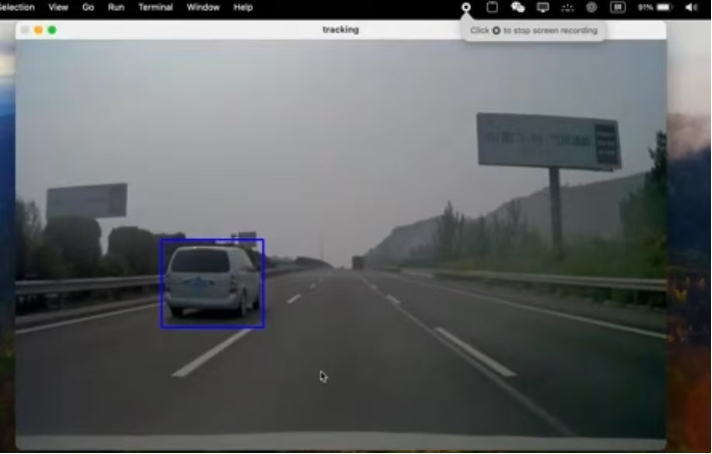
\includegraphics[width=0.5\linewidth]{img/kcf-target-selection.png}
  \caption{\label{fig:kcf_select}\textit{Initial target selection using manual bounding box.}}
\end{figure}
\begin{figure}
  \centering
  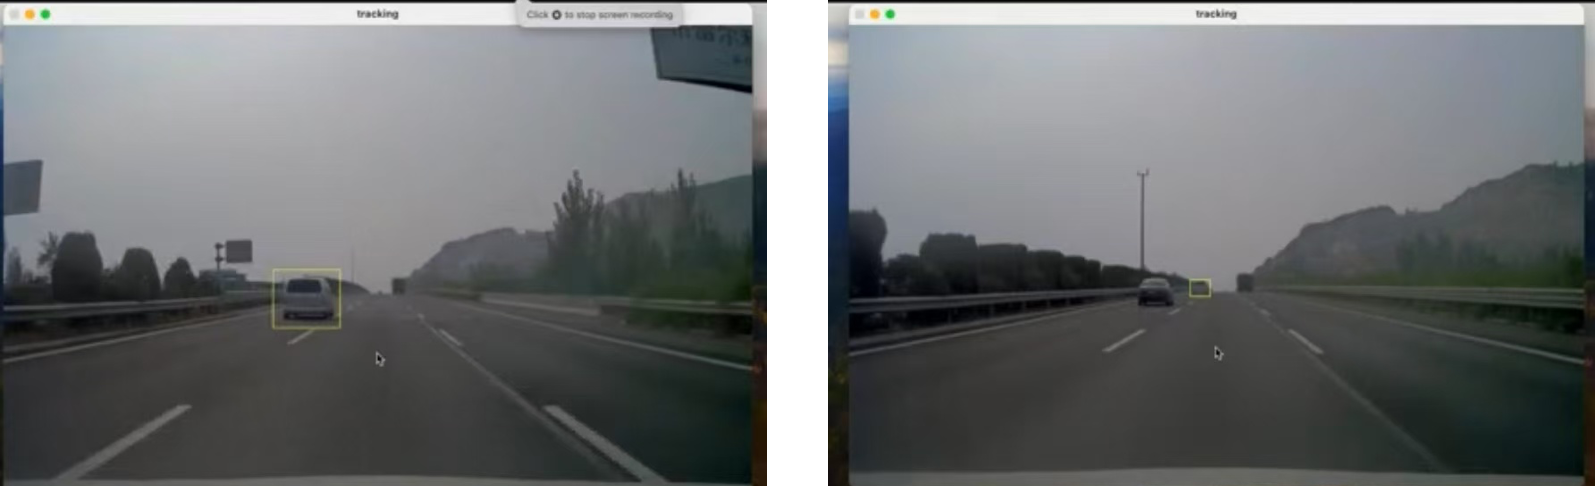
\includegraphics[width=1\linewidth]{img/kcf-position-updates.png}
  \caption{\label{fig:kcf_updates}\textit{Target position updates using the KCF tracker.}}
\end{figure}

\subsubsection{Voting/Stacking Module}

The initial experiment on the voting and stacking modules is implemented separately but within the same framework in MATLAB. In the voting module, multiple tracking models, each producing predictions like bounding boxes or keypoints, are integrated using a majority voting method to determine the final object position for each frame. In the stacking module, the predictions from the base trackers are used to form feature vectors, which are then input into a meta-model for training to optimize the final tracking result. The code for both experiments is written in MATLAB, and these two methods are being explored separately to compare their performance and effectiveness in improving tracking accuracy.

% -------------------------- CONCLUSION AND FUTURE WORK --------------------------

\section{Conclusion and Future Work}

In this literature review, we explored the evolution of single object tracking (SOT) techniques, starting with traditional feature based methods such as Histogram of Oriented Gradients(HOG) and Scale-Invariant Feature Transform (SIFT). While these techniques offer strong feature extraction capabilities, they are computationally expensive and lack robustness in dynamic tracking environments.

Correlation filter approaches track frames in the frequency domain. Discriminative Correlation Filters (DCF) introduced supervised learning principles which improved performance, but it suffers from boundary effects. Spatially Regularized DCF(SRDCF) mitigates these effects by penalizing background regions, enhancing object discrimination. Kernelized Correlation Filters (KCF) further optimize feature representations by incorporating nonlinear kernel methods, although it is limited by a fixed scale. MOSSE tracking stands out for its high speed and adaptability, but is prone to drift and occlusion sensitivity. Continuous Convolution Operators Tracker (CCOT) introduced multi-resolution deep feature maps, which overcomes the single resolution limitations of previous DCF based methods. We also looked at the Discriminative Scale Space Tracker(DSST) to address scale variation in SOT. This method introduces a dedicated scale filter alongside the traditional translation filter. This improves robustness, especially to resizing and occlusion.

Ensemble models for object tracking, though less explored in research, have demonstrated promise in combining strengths of multiple tracking techniques. Based on these findings, our proposed model will integrate MOSSE, CCOT, KCF, DSST and DCF using ensemble strategies such as stacking and voting. The voting approach will combine tracking results from individual models, while stacking will use a meta-model to learn optimal combinations of base model predictions. By leveraging the complementary strengths of these trackers, our approach aims to enhance robustness against scale variation, motion blur, occlusion and background clutter.

Going forward, we will implement and evaluate our proposed ensemble-based object tracking system.

\begin{itemize}
  \item Developing an integrated framework that runs MOSSE, CCOT, KCF, DSST and DCF.
  \item Implementing stacking and voting strategies to determine the most effective ensemble approach.
  \item Conducting experimental evaluations on benchmark datasets to assess tracking performance, accuracy, robustness and computational efficiency.
  \item Exploring potential optimizations, including additional feature fusion techniques to enhance tracking performance.
\end{itemize}

By the end of this development cycle, we aim to produce an efficient, high performance object tracking system capable of handling real world challenges in SOT. The insights gained from this work may also be used to inform future research directions, particularly in extending ensemble methods for real time object tracking applications.

% -------------------------- REFERENCES --------------------------

\clearpage
\bibliographystyle{IEEEtran}
\bibliography{refs}

\end{document}